\documentclass{beamer}
\usetheme{CambridgeUS}
\usepackage{graphicx}
\usepackage{booktabs}
\usepackage{amsmath}
\usepackage{tikz}
\usepackage{listings}
\usepackage{xcolor}
\definecolor{nebulablue}{RGB}{25,118,210}
\definecolor{nebulagray}{RGB}{97,97,97}

\title[Nebula GPU Interconnect]{Nebula GPU Interconnect System:\\Technical Architecture and Implementation}
\author{Pranav Chandra, Pramit Pal, Meghadri Ghosh\\Team Bob}
\date{September 2025}

\begin{document}

%-------------------------------------------------
\begin{frame}
  \titlepage
\end{frame}

%-------------------------------------------------
\begin{frame}{Project Overview}
  \begin{itemize}
    \item \textbf{Goal:} Scalable, cache-coherent GPU interconnect for AI/ML workloads
    \item \textbf{Topology:} 2D mesh, 2x2 to 8x8 grid (up to 64 GPUs)
    \item \textbf{Protocols:} ARM AMBA AXI4 (non-coherent), CHI (coherent)
    \item \textbf{Implementation:} SystemVerilog RTL, Python analysis, Web dashboard
    \item \textbf{Key Features:}
      \begin{itemize}
        \item Five-stage router pipeline with virtual channels
        \item Adaptive and deterministic routing
        \item Protocol translation bridges (AXI4/CHI $\leftrightarrow$ NoC)
        \item Performance monitoring and visualization
      \end{itemize}
  \end{itemize}
\end{frame}

%-------------------------------------------------
\begin{frame}{System Architecture}
%  \begin{figure}
%    \centering
%    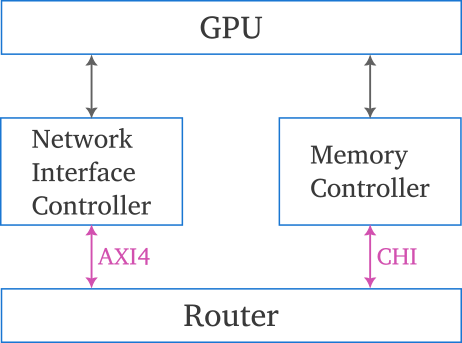
\includegraphics[width=0.7\linewidth]{images/component-architecture.png}
%    \caption{Nebula System Component Architecture}
%  \end{figure}
  \begin{itemize}
    \item Mesh topology generated by \texttt{nebula\_mesh\_top.sv}
    \item Routers interconnected, edge nodes terminated
    \item Each node: router + protocol bridge + GPU/memory interface
  \end{itemize}
\end{frame}

%-------------------------------------------------
\begin{frame}{Router Microarchitecture}
  \textbf{Five-Stage Pipeline:}
  \begin{enumerate}
    \item Buffer Write (BW): Input port, VC allocation
    \item Route Computation (RC): XY/adaptive routing
    \item Virtual Channel Allocation (VA): VC state machines, credit reservation
    \item Switch Allocation (SA): Crossbar arbitration, fairness
    \item Switch Traversal (ST): Data transmission, credit management
  \end{enumerate}
  \vspace{0.5em}
  \textbf{Features:}
  \begin{itemize}
    \item 4 VCs per port, 16-flit FIFO depth
    \item Credit-based flow control
    \item Round-robin arbitration
    \item Congestion-aware adaptive routing
  \end{itemize}
\end{frame}

%-------------------------------------------------
\begin{frame}{Routing Algorithms}
  \begin{itemize}
    \item \textbf{XY Routing:} Dimension-ordered, deadlock-free
    \item \textbf{Adaptive Routing:} Congestion-aware, selects least congested path
    \item \textbf{Implementation:}
      \begin{itemize}
        \item Combinational logic compares router and destination coordinates
        \item Congestion metrics: buffer utilization, credit counts
        \item Programmable thresholds for adaptive switching
      \end{itemize}
  \end{itemize}
  \begin{block}{Technical Details}
    \begin{itemize}
      \item Route Computation: lines 260-380 in \texttt{nebula\_router.sv}
      \item VC Allocation: lines 630-690 in \texttt{nebula\_router.sv}
      \item Switch Allocation: lines 460-570 in \texttt{nebula\_router.sv}
    \end{itemize}
  \end{block}
\end{frame}

%-------------------------------------------------
\begin{frame}{Flit and Packet Format}
  \begin{itemize}
    \item \textbf{Flit:} 256 bits, defined in \texttt{nebula\_pkg.sv}
    \item \textbf{Header Fields:}
      \begin{itemize}
        \item Type (HEAD/BODY/TAIL/SINGLE)
        \item Source/Dest coordinates (4 bits each)
        \item VC ID (2 bits)
        \item Sequence number (16 bits)
        \item Packet ID (8 bits)
        \item QoS (4 bits)
        \item CRC (32 bits)
      \end{itemize}
    \item \textbf{Payload:} 208 bits
    \item \textbf{Multi-flit packets:} HEAD, BODY, TAIL; single-flit packets supported
  \end{itemize}
\end{frame}

%-------------------------------------------------
\begin{frame}{Protocol Translation Bridges}
  \begin{itemize}
    \item \textbf{AXI-NoC Bridge (\texttt{nebula\_axi\_noc\_bridge.sv}):}
      \begin{itemize}
        \item Burst decomposition, address mapping
        \item 64-entry reorder buffer
        \item Packet assembly/disassembly
        \item Error detection, latency monitoring
      \end{itemize}
    \item \textbf{CHI-NoC Bridge (\texttt{nebula\_chi\_noc\_bridge.sv}):}
      \begin{itemize}
        \item CHI message classification, VC mapping
        \item Directory-based MOESI coherency
        \item Snoop response aggregation
        \item Timeout/error handling
      \end{itemize}
    \item \textbf{Outstanding Transaction Management:}
      \begin{itemize}
        \item Hardware table tracks up to 64 operations
        \item Transaction ID, address, burst length, sequence, timeout
      \end{itemize}
  \end{itemize}
\end{frame}

%-------------------------------------------------
\begin{frame}{Packet Assembly and Disassembly}
  \begin{itemize}
    \item \textbf{Assembler (\texttt{nebula\_packet\_assembler.sv}):}
      \begin{itemize}
        \item Converts protocol transactions to flit packets
        \item Header generation, payload segmentation
        \item Address-to-coordinate mapping
      \end{itemize}
    \item \textbf{Disassembler (\texttt{nebula\_packet\_disassembler.sv}):}
      \begin{itemize}
        \item Reconstructs transactions from flits
        \item CRC verification, sequence management
        \item Handles out-of-order and multi-path delivery
      \end{itemize}
  \end{itemize}
\end{frame}

%-------------------------------------------------
\begin{frame}{Credit-Based Flow Control}
  \begin{itemize}
    \item \textbf{Credit Controller (\texttt{nebula\_credit\_flow\_ctrl.sv}):}
      \begin{itemize}
        \item Per-VC credit counters, max 16
        \item Increment on flit acceptance, decrement on allocation
        \item Prevents buffer overflow, deadlock
        \item \texttt{credits\_available} signals for arbitration
      \end{itemize}
    \item \textbf{Flow Control Protocol:}
      \begin{itemize}
        \item Sender stalls if credits = 0
        \item Lossless operation guaranteed
      \end{itemize}
  \end{itemize}
\end{frame}

%-------------------------------------------------
\begin{frame}{System Integration}
  \begin{itemize}
    \item \textbf{Top-Level Modules:}
      \begin{itemize}
        \item \texttt{nebula\_system\_top.sv}: Mesh instantiation, AXI4 interfaces, address mapping
        \item \texttt{nebula\_mesh\_top.sv}: Router grid generation, edge handling
        \item \texttt{nebula\_top.sv}: Configuration registers, system status, debug
      \end{itemize}
    \item \textbf{Address Mapping:}
      \begin{itemize}
        \item 64-bit global address space
        \item Static/dynamic schemes (partitioning, hashing)
        \item Hardware decoder for coordinate extraction
      \end{itemize}
    \item \textbf{Collective Operations:}
      \begin{itemize}
        \item Broadcast/multicast via packet replication
        \item Hardware barriers, reduction support
      \end{itemize}
  \end{itemize}
\end{frame}

%-------------------------------------------------
\begin{frame}{Verification and Testing}
  \begin{itemize}
    \item \textbf{RTL Testbenches (\texttt{code/tb/}):}
      \begin{itemize}
        \item Unit tests: packet assembler/disassembler, FIFO, arbiter
        \item Integration tests: AXI-NoC bridge, router, mesh
        \item System-level: end-to-end, multi-hop, congestion, performance
      \end{itemize}
    \item \textbf{Python Tools:}
      \begin{itemize}
        \item \texttt{nebula\_traffic\_generator.py}: Traffic pattern generation, testbench synthesis
        \item \texttt{nebula\_vcd\_parser.py}: VCD trace analysis, packet event extraction
      \end{itemize}
    \item \textbf{Metrics:}
      \begin{itemize}
        \item Latency, throughput, congestion, error rates
        \item Performance counters in routers and system top
      \end{itemize}
  \end{itemize}
\end{frame}

%-------------------------------------------------
\begin{frame}{Web Dashboard}
  \begin{itemize}
    \item \textbf{Backend:} Flask + Socket.IO (\texttt{web\_dashboard/backend/app.py})
    \item \textbf{Frontend:} Vanilla JS + Vite + Tailwind (\texttt{web\_dashboard/frontend/})
    \item \textbf{Features:}
      \begin{itemize}
        \item Real-time mesh visualization (SVG)
        \item Animated packet flows, congestion heatmap
        \item Performance metric graphing (utilization, latency, throughput)
        \item VCD trace replay, simulation control
        \item Traffic pattern selection (Uniform, Hotspot, CNN, Matrix, Transformer, etc.)
      \end{itemize}
    \item \textbf{Integration:}
      \begin{itemize}
        \item Runs Verilog simulations, parses VCD, updates UI via WebSocket
        \item API endpoints for mesh, performance, simulation control
      \end{itemize}
  \end{itemize}
\end{frame}

%-------------------------------------------------
\begin{frame}{Performance Monitoring}
  \begin{itemize}
    \item \textbf{Router-Level Counters:}
      \begin{itemize}
        \item Packets forwarded per direction
        \item Buffer utilization, VC statistics
        \item Congestion, temperature (simulated)
      \end{itemize}
    \item \textbf{System-Level Metrics:}
      \begin{itemize}
        \item Total packets routed, average latency, throughput
        \item Error and protocol violation tracking
        \item Historical trending for optimization
      \end{itemize}
    \item \textbf{Visualization:}
      \begin{itemize}
        \item Time-series graphs, mesh overlays
        \item VCD replay for cycle-accurate analysis
      \end{itemize}
  \end{itemize}
\end{frame}

%-------------------------------------------------
\begin{frame}{Technical Challenges}
  \begin{itemize}
    \item \textbf{Scalability:} Mesh generation, address mapping for large grids
    \item \textbf{Coherency:} CHI protocol edge cases, directory state management
    \item \textbf{Adaptive Routing:} Congestion metrics, deadlock avoidance
    \item \textbf{Verification:} Multi-level test coverage, error injection
    \item \textbf{Integration:} Protocol bridge correctness, performance counter aggregation
    \item \textbf{Visualization:} Real-time updates, VCD parsing, UI responsiveness
  \end{itemize}
\end{frame}

%-------------------------------------------------
\begin{frame}{Current Status and Future Work}
  \begin{itemize}
    \item \textbf{Completed:}
      \begin{itemize}
        \item Mesh topology, router pipeline, protocol bridges
        \item AXI4/CHI support, packet assembler/disassembler
        \item Python traffic generator, VCD parser, web dashboard
        \item Verification infrastructure, performance monitoring
      \end{itemize}
    \item \textbf{In Progress:}
      \begin{itemize}
        \item Advanced adaptive routing, QoS features
        \item Hierarchical clustering, multi-mesh support
        \item Enhanced CHI edge case handling
        \item Dashboard UI improvements, analytics
      \end{itemize}
    \item \textbf{Planned:}
      \begin{itemize}
        \item FPGA prototyping, hardware deployment
        \item Deep learning workload benchmarks
        \item Fault tolerance, dynamic reconfiguration
      \end{itemize}
  \end{itemize}
\end{frame}

%-------------------------------------------------
\begin{frame}{References}
  \begin{itemize}
    \item SystemVerilog RTL: \texttt{code/rtl/}
    \item Python Tools: \texttt{code/python/}
    \item Testbenches: \texttt{code/tb/}
    \item Documentation: \texttt{docs/final\_report.tex}, \texttt{docs/abstract.tex}
    \item Dashboard: \texttt{web\_dashboard/}
  \end{itemize}
\end{frame}

%-------------------------------------------------
\begin{frame}{Q\&A}
  \centering
  \Huge Questions?
\end{frame}

\end{document}